\documentclass{article}

% set font encoding for PDFLaTeX, XeLaTeX, or LuaTeX
\usepackage{ifxetex}
\ifxetex
  \usepackage{fontspec}
\else
  \usepackage[T1]{fontenc}
  \usepackage[utf8]{inputenc}
  \usepackage{lmodern}
  \usepackage{graphicx}
  \usepackage{siunitx}
  \usepackage{amsmath}
  \usepackage{float}
\fi

% used in maketitle
\usepackage[left=3cm,right=3cm,top=3cm,bottom=3cm]{geometry}
\title{Actividad 7}
\author{Luis Aarón Cerón Ramírez}

% Enable SageTeX to run SageMath code right inside this LaTeX file.
% documentation: http://mirrors.ctan.org/macros/latex/contrib/sagetex/sagetexpackage.pdf
% \usepackage{sagetex}

\begin{document}
\maketitle
\section{Introducción}
En esta actividad se continua con el texto de Fay y Graham de resortes acoplados, las secciones 3 y 4 sobre un sistema de resortes no lineales y forzados.
En la sección 3 se tienen resortes que ya no cumplen la Ley de Hooke, sino que se comportan como un sistema no lineal.
Mientras que la sección 4 impone un forzamiento periódico sobre el sistema oscilador de masas.

\section{Marco teórico}
\subsection{Adicionando la no linealidad}
Si asumimos que la fuerza de restitución es no lineal, la cuál es para grandes vibraciones.
\newline
En este caso en vez de considerar la fuerza de restitución como $-kx$ (Ley de Hooke), suponemos que este es de la forma $-kx$+$\mu x^3$. Por lo que nuestro modelo se convierte en
\begin{equation}
\begin{aligned}
\\m_1\ddot x_1= -\delta_1\dot x_1-k_1x_1+\mu_1x_1^{3}-k_2(x_1-x_2)+\mu_2(x_1-x_2)^3\\
\\m_2\ddot x_2= -\delta_2\dot x_2-k_2(x_2-x_1)+\mu_2(x_2-x_1)^3\\
\end{aligned}
\end{equation}
En este caso el rango de movimiento para un modelo no lineal es mucho mas complicado que del modelo lineal.

\subsection{Adicionando el forzamiento}
Es una cuestión tan simple como agregar el forzamiento externo al modelo, asumiendo un forzamiento senoídal de la forma F$\cos(wt)$, por lo que el modelo queda de la siguiente forma:
\begin{equation}
\begin{aligned}
\\m_1\ddot x_1= -\delta_1\dot x_1-k_1x_1+\mu_1x_1^{3}-k_2(x_1-x_2)+\mu_2(x_1-x_2)^3+F_1\cos(w_1t)\\
\\m_2\ddot x_2= -\delta_2\dot x_2-k_2(x_2-x_1)+\mu_2(x_2-x_1)^3+F_2\cos(w_2t)\\
\end{aligned}
\end{equation}
El rango de movimiento para este caso es mas vasto. Podemos encontrar soluciones limitadas y sin limites(resonancia no lineal), soluciones periódicas que comparten el periódo con el forzamiento(soluciones armónicas) y soluciones que son periódicas del periódo en múltiplos y soluciones de estados estacionarios. Algo importante que hay que mencionar es que las condiciones bajo las cuales ocurren estos movimientos no son facíles de establecer.

\section{Resultados}
Se anexan las grafícas reproducidas en jupyter lab

\begin{figure}[H]
\centering
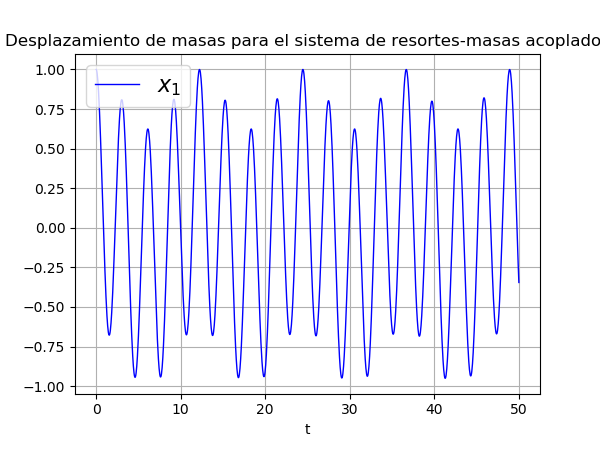
\includegraphics[scale=0.59]{31_d1.png}
\end{figure}

\begin{figure}[H]
\centering
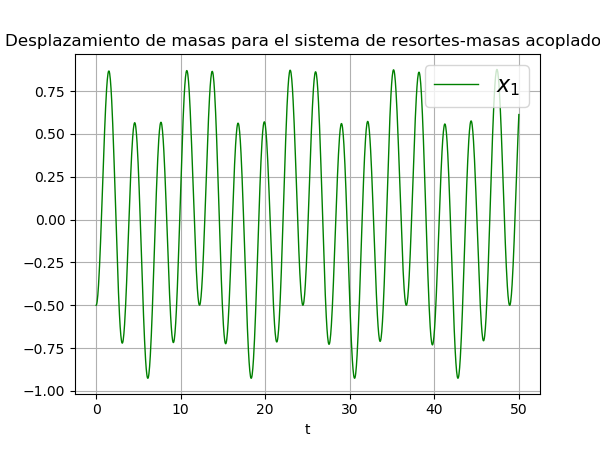
\includegraphics[scale=0.59]{31_d2.png}
\end{figure}

\begin{figure}[H]
\centering
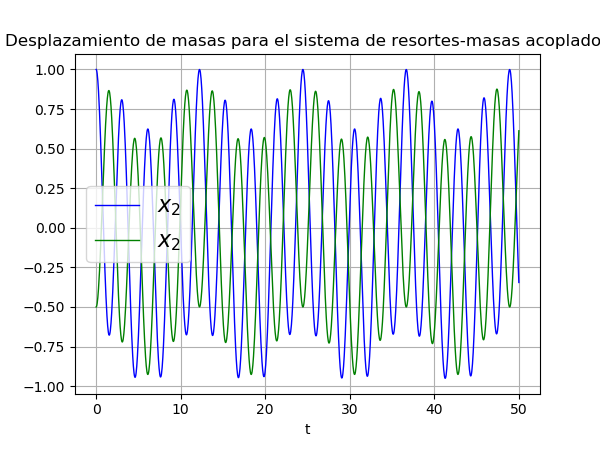
\includegraphics[scale=0.59]{31_d12.png}
\end{figure}

\begin{figure}[H]
\centering
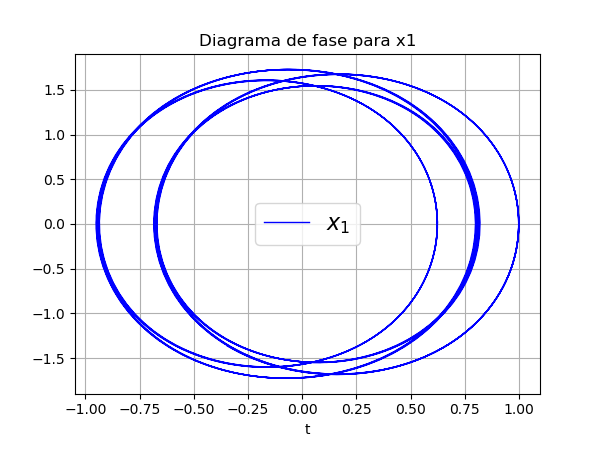
\includegraphics[scale=0.59]{31_f1.png}
\end{figure}

\begin{figure}[H]
\centering
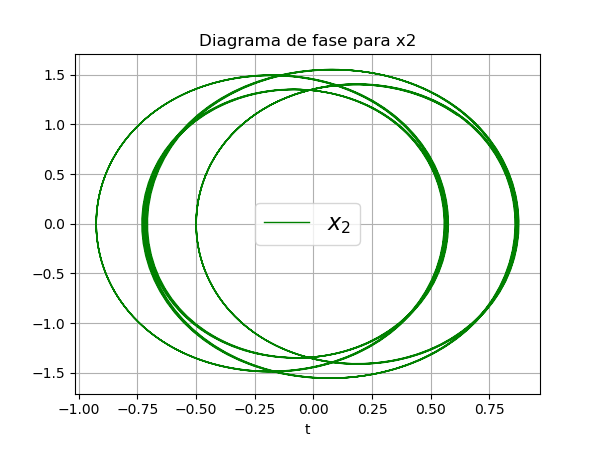
\includegraphics[scale=0.59]{31_f2.png}
\end{figure}

\begin{figure}[H]
\centering
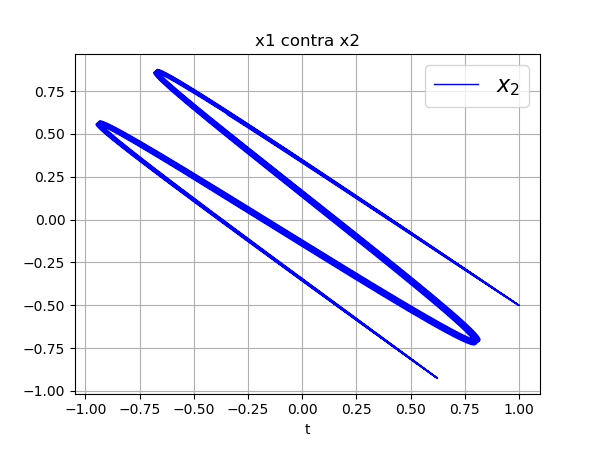
\includegraphics[scale=0.59]{31_v.png}
\end{figure}

\begin{figure}[H]
\centering
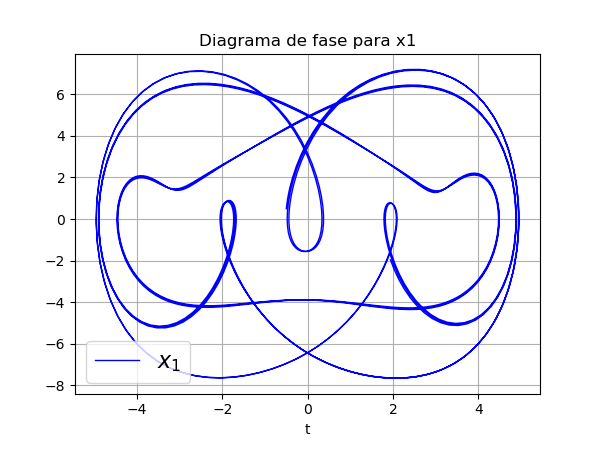
\includegraphics[scale=0.59]{32_f1.png}
\end{figure}

\begin{figure}[H]
\centering
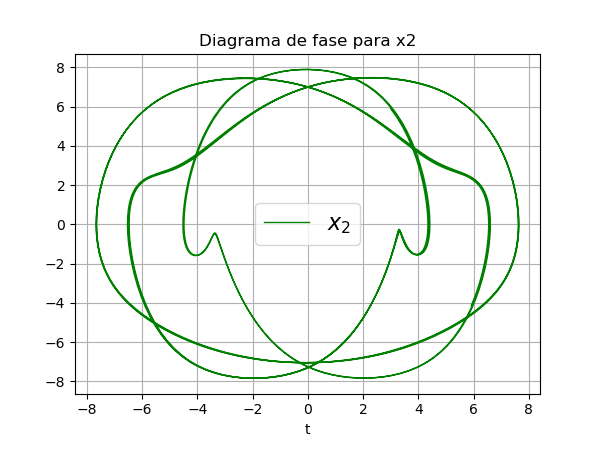
\includegraphics[scale=0.59]{32_f2.png}
\end{figure}

\begin{figure}[H]
\centering
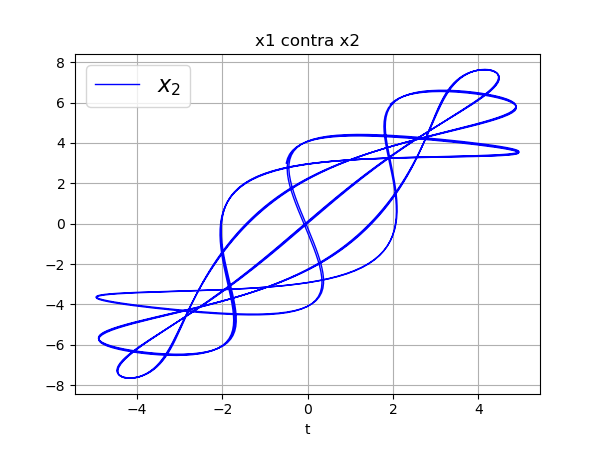
\includegraphics[scale=0.59]{32_v.png}
\end{figure}

\begin{figure}[H]
\centering
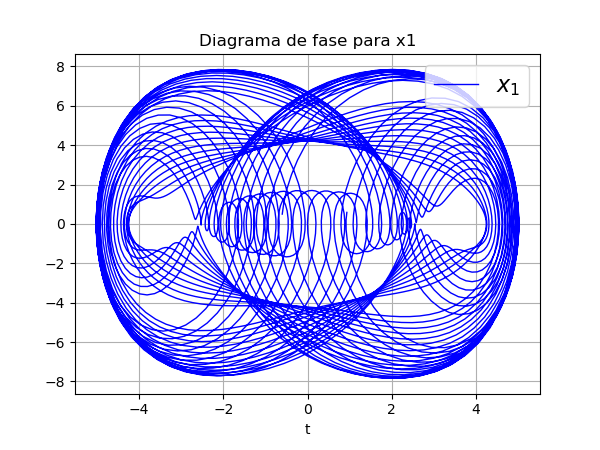
\includegraphics[scale=0.59]{33_f1.png}
\end{figure}

\begin{figure}[H]
\centering
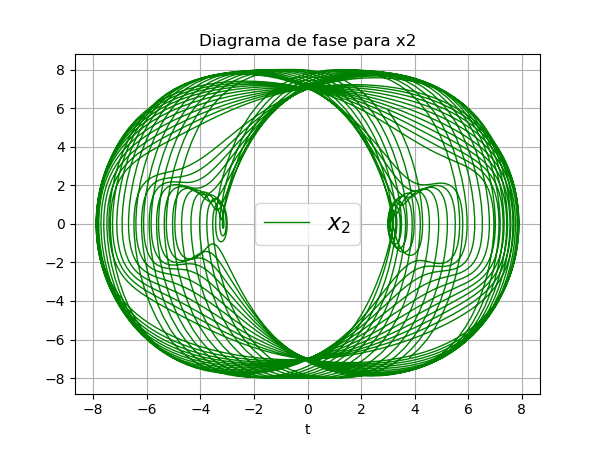
\includegraphics[scale=0.59]{33_f2.png}
\end{figure}

\begin{figure}[H]
\centering
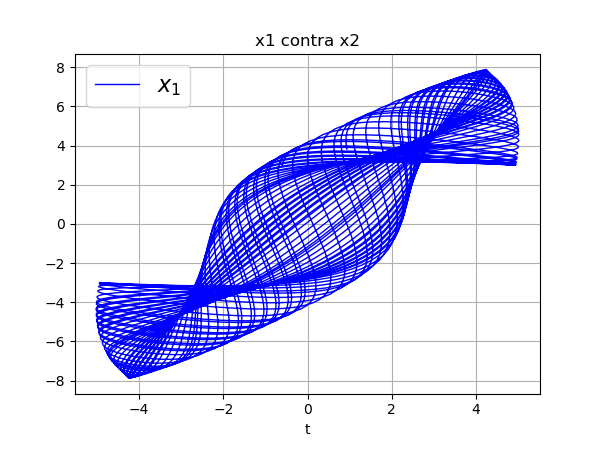
\includegraphics[scale=0.59]{33_v.png}
\end{figure}

\begin{figure}[H]
\centering
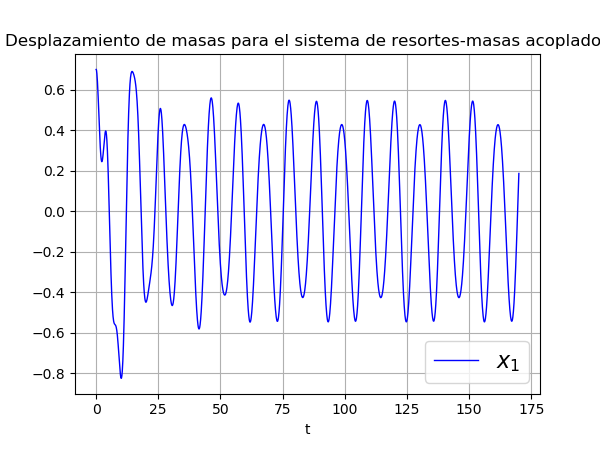
\includegraphics[scale=0.59]{41_d1.png}
\end{figure}

\begin{figure}[H]
\centering
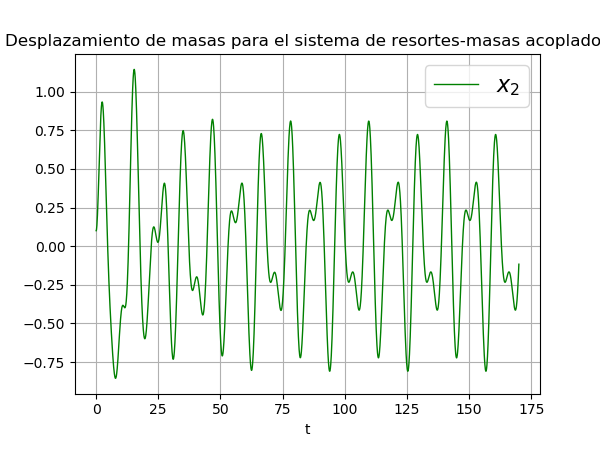
\includegraphics[scale=0.59]{41_d2.png}
\end{figure}

\begin{figure}[H]
\centering
\includegraphics[scale=0.59]{41_d12.png}
\end{figure}

\begin{figure}[H]
\centering
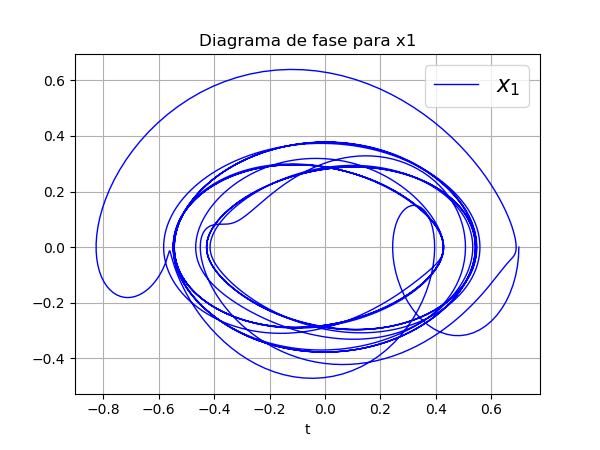
\includegraphics[scale=0.59]{41_f1.png}
\end{figure}

\begin{figure}[H]
\centering
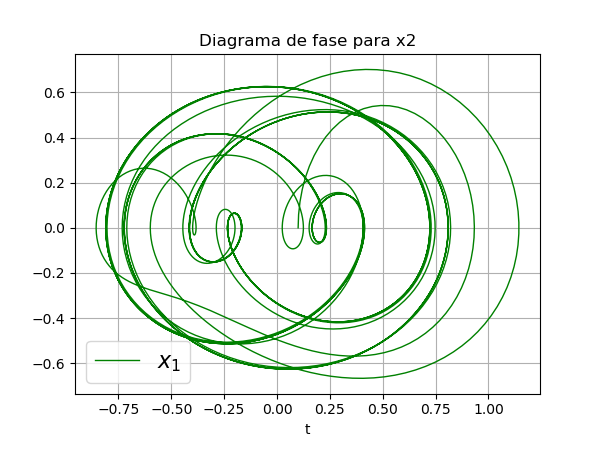
\includegraphics[scale=0.59]{41_f2.png}
\end{figure}

\begin{figure}[H]
\centering
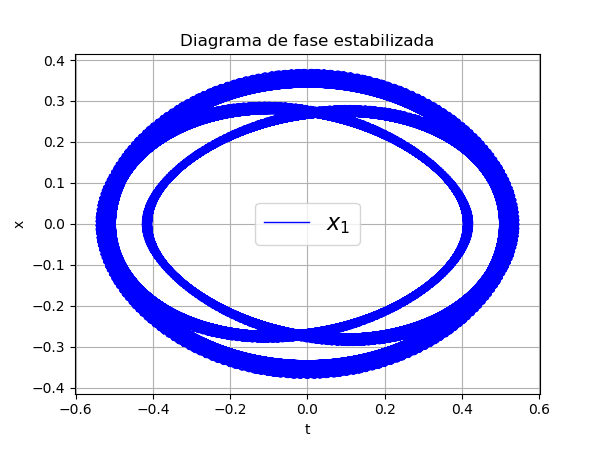
\includegraphics[scale=0.59]{41_fe1.png}
\end{figure}

\begin{figure}[H]
\centering
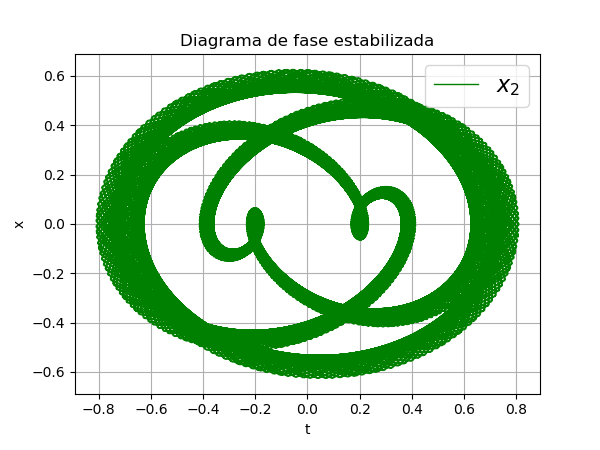
\includegraphics[scale=0.59]{41_fe2.png}
\end{figure}

\begin{figure}[H]
\centering
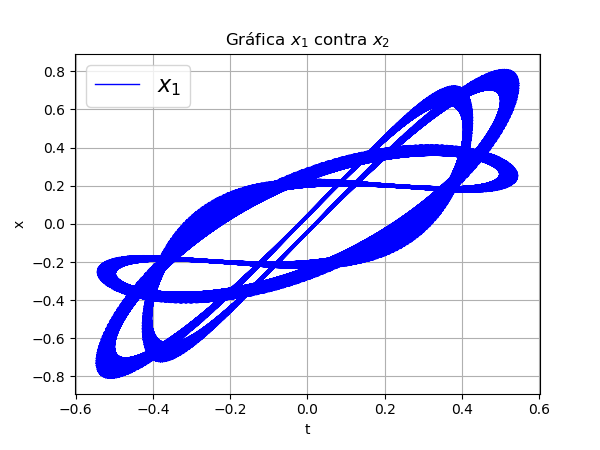
\includegraphics[scale=0.59]{41.png}
\end{figure}

\section{Conclusión}
Se puede concluir lo mismo que en el trabjo anterior, ya que este trabajo es una continuación del texto de Fay y Graham, por lo que volvimos a observar la importancia de las herramientas computacionales para resolver problemas que en caso de hacer a mano serian muy tediosos, así como la utilidad para visualizar por medio de grafícas los comportamientos descritos en las ecuaciones.

\section{Apendice}
¿Qué más te llama la atención de la actividad completa?
\newline
La facilidad con que se puede reproducir las graficas
\newline
¿Que se te hizo menos interesante?
\newline
El tener que hacer el codigo
\newline
¿De un sistema de masas acopladas como se trabaja en esta actividad, hubieras pensado que abre toda una nueva área de fenómenos no lineales?
\newline
Habia escuchado un poco al respecto, pero ahondado en el tema, me parece muy interesante la diferencia al estudiar los comportamientos del sistema y me gustaría estudiar mas
\newline
¿Qué propondrías para mejorar esta actividad?
\newline
Mas modelos
\newline
¿Te ha parecido interesante este reto?
\newline
si, aunque he tenido problemas para colocar las imagenes
\newline
¿Quisieras estudiar mas este tipo de fenómenos no lineales?
\newline
Si, me gustaria una practica donde se hablara sobre atractores


\end{document}
